\newpage
\chapter{Literature Review}
\section{Introduction}
This chapter reviews the literature to provide background information on the theory of tracking filters in \ac{Radar} Target Tracking and Passive \ac{Radar} systems. The history of tracking filters in \ac{Radar} traces back to the early days of \ac{Radar} technology during World War II, when the need for accurate tracking became paramount. In the late 1950s, Rudolph Kalman developed his theory on the Kalman Filter, which revolutionised the domain of control theory. In 2008, Kalman was awarded the Draper Prize from the National Engineering Academy for his work on the filter \cite{kalmanNAE}. The Kalman Filter was used in the Apollo project for navigation, where accurate estimates for trajectories of manned spacecraft were required and it proved to be ideal for providing estimates in real-time \cite{Andrews2010}.

As computer technology advanced, tracking filters have evolved from the Kalman Filter to more advanced estimation techniques such as the Kalman Filter variants like \ac{EKF} and \ac{UKF} and other various filters to be discussed. This evolution has been driven by the increasing complexity of tracking needs in \ac{Radar} tracking systems, which have migrated from ground-based systems in the past to airborne systems and to tracking systems on missiles currently \cite{Andrews2010}. These more advanced filters are better equipped to handle non-linear dynamics of targets, Non-Gaussian process noise and measurement noise.

The theory review briefly discusses an overview of \ac{PR} systems, state estimation, various tracking filters used across multiple domains, as well as techniques for adaptive and multi-target tracking. The tracking filters are discussed in depth, with a focus on tracking filters that are better equipped to handle the tracking problem of aircraft in the bistatic range and Doppler domain. Furthermore, different performance metrics used to evaluate tracking filters are reviewed as well as techniques for multi-target tracking and clustering from a \ac{CFAR} Map. To comprehensively understand the application of tracking filters in \ac{PR} systems, an overview of  \ac{PR} systems is provided.
%%%%%%%%%%%%%%%%%%%%%%%%%%%%%%%%%%%%%%%%%%%%%%%%%%%%%%%%%%%%%
%%\subsection{Tracking concepts}
\subsection{Passive Radar Systems}
The concept of using \ac{PR} measurements for aircraft detection dates back to 1935, when Sir Robert Watson-Watt carried out a pioneering bistatic experiment where he utilized ``the shortwave (49 m wavelength) BBC Empire transmitter at Daventry to detect a Heyford bomber aircraft at a distance of 8 km'', as noted by R.V. Jones \cite{Jones1986}. Following a successful demonstration of the experiment, the Bawdsey Research Station was established as a new \ac{Radar} research establishment under the Air Ministry with Sir Robert Watson-Watt as the superintendent in 1936 \cite{Kuschel2010a}.

Later, his research resulted in the establishment of a series of radars along the south and east coasts of England, referred to as the Chain Home radars, whose sole function was to serve as an early warning system \cite{Jones1986}. In 1943, the German "Klein Heidelberg" receivers were developed as the first operational \ac{PR} system as observed in Figure \ref{fig1:klein} \cite{Colone2023}. Figure \ref{fig1:klein} from \cite{Willis2007} depicts a constant range-sum ellipse, illustrating the bistatic detection area. The Chain Home Radars operated in an active mode, emitting signals with a power output of 350 kW, which was later upgraded to 750 kW, and operated within a frequency range of 20 to 30 MHz \cite{Kuschel2010a}. Meanwhile, on the German side, passive radar systems were strategically positioned along the continental coast of the Channel \cite{Kuschel2010a}. They detected aircraft using emissions from the British "Chain Home" \ac{Radar}s without transmitting, making them advantageous due to their resistance to jammers. 

\begin{figure}[ht!]
	\centering
	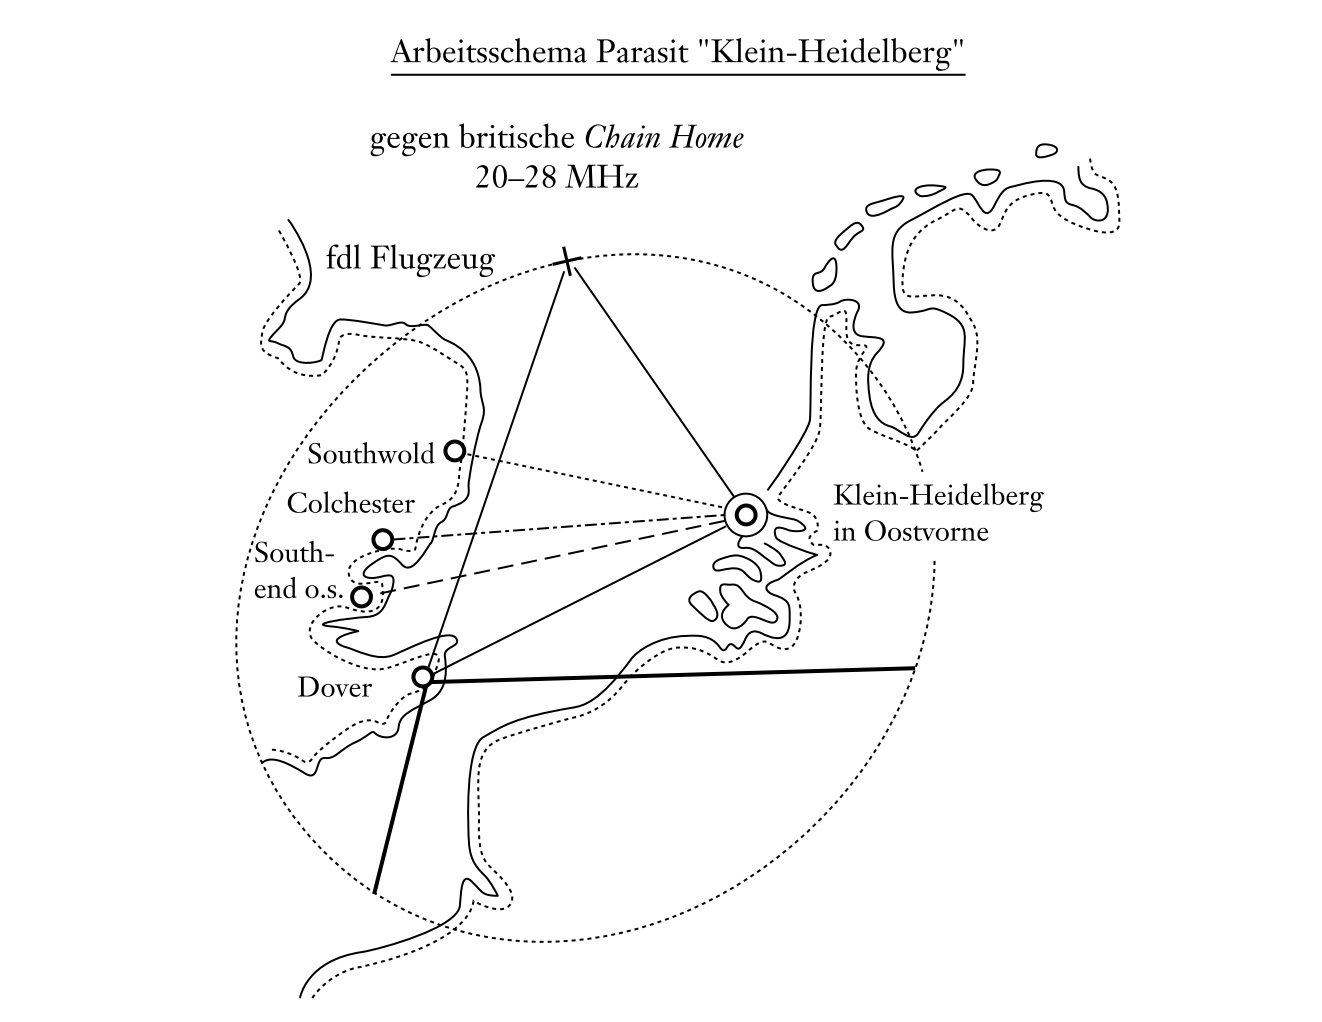
\includegraphics[width=0.85\linewidth]{Figure/KHeid.png}
	\caption{Sketch of the Klein Heidelberg (KH) geometry.}
	\label{fig1:klein}
\end{figure}

After World War II, there has been a lot of extensive research on \ac{PR}. The elimination of a dedicated transmitter requirement and the use of commercially available ready-made components has enabled numerous universities and research institutions to create experimental setups \cite{Colone2023}. Following these developments, Lockheed Martin pioneered the prototype development of the earliest \ac{PR} \ac{FM}-radio broadcasts \cite{Kuschel2010a}, succeeded by further developments from industry and research institutions.

%%%% Definiton of the basic prinicples in Passive \ac{Radar}
\ac{PR} systems are a type of \ac{Radar} that utilize non-cooperative or cooperative illuminators of opportunity, such as commercial broadcasts (\ac{FM}, \ac{DAB},
and \ac{DVB-T/T2}), cellular signals, \ac{WiFi}, and satellite-borne transmitters (\ac{GNSS}, \ac{DVB-S/S2}), to detect and track objects. \ac{PR} systems do not emit any signals but rely on the reflections from targets illuminated by signals from other transmitters(illuminators of opportunity). The principle of \ac{PR}  is based on cross-correlating a signal directly received from the transmitter and signal reflected from the target \cite{Kuschel2010a}. Figure  \ref{fig1:multistatic} illustrates a multi-static \ac{PR} system from \cite{mltistaticRadar}.
%diagram to illustrate a passive \ac{Radar} system.

\begin{figure}[ht!]
	\centering
	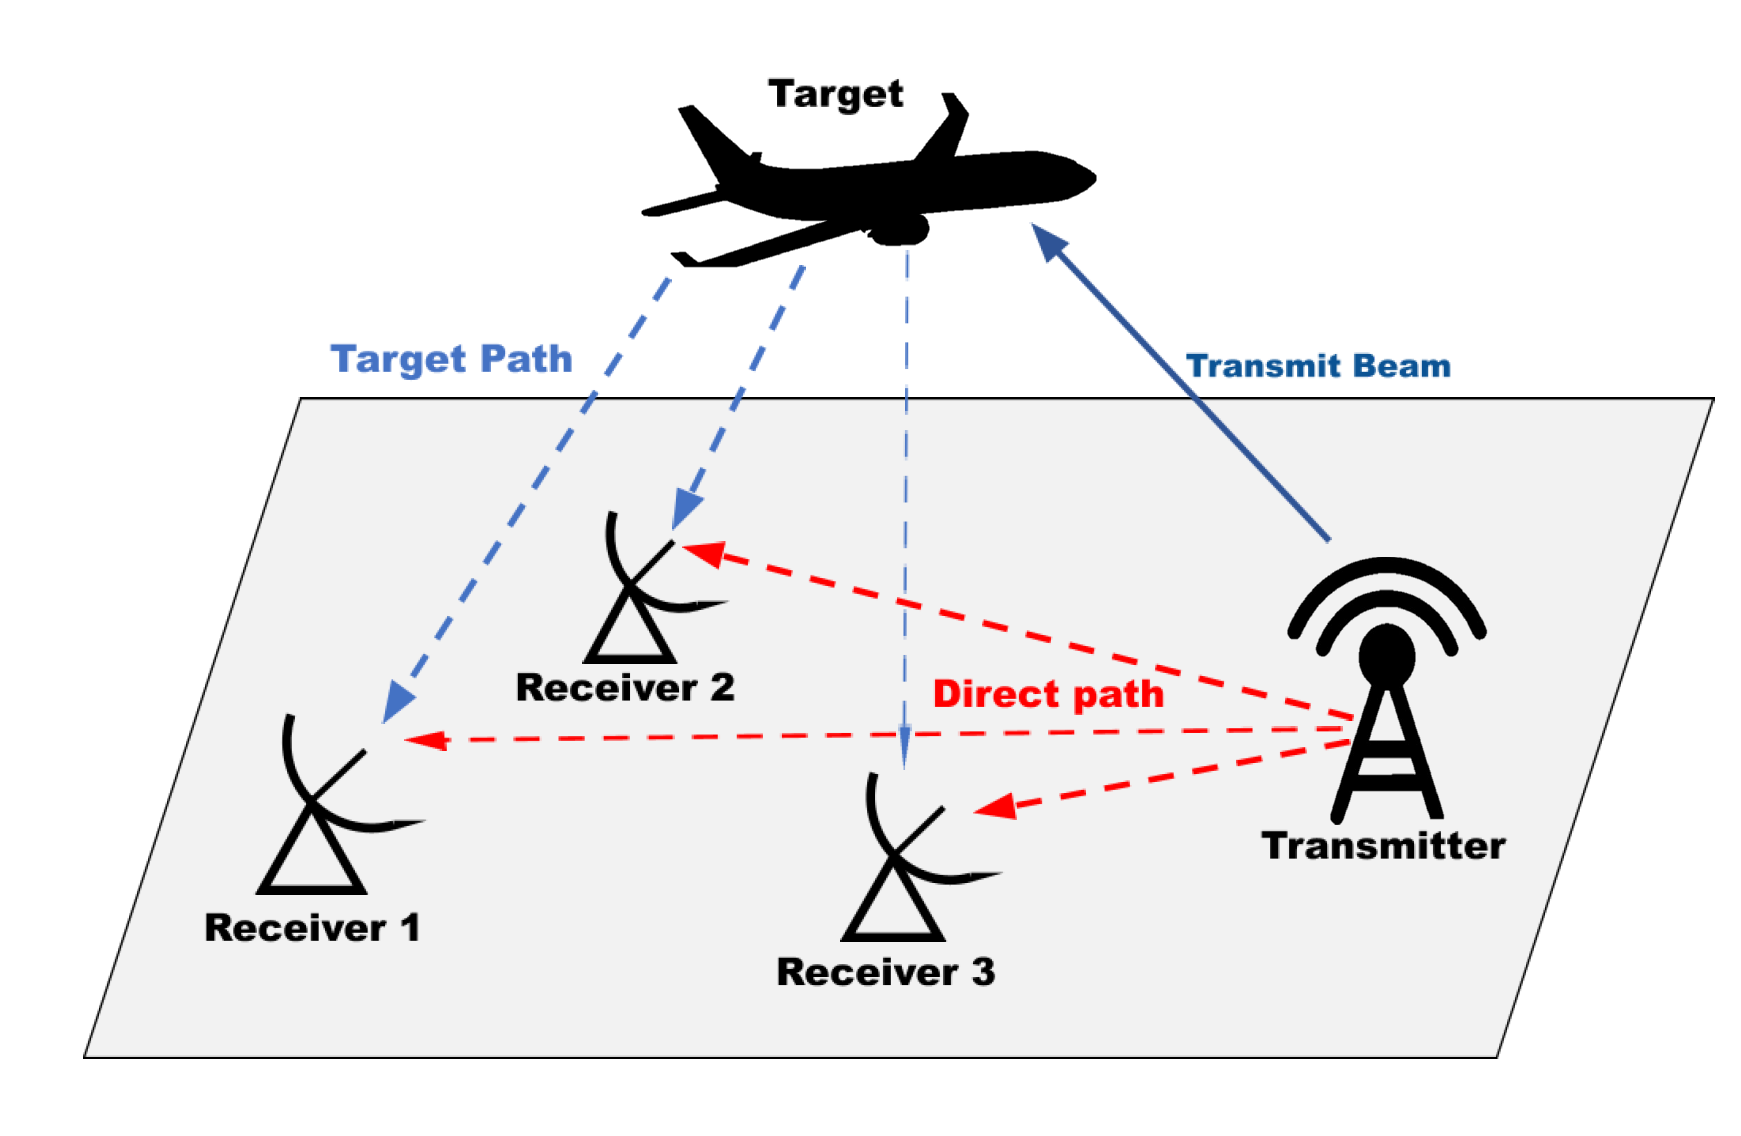
\includegraphics[width=0.9\linewidth]{Figure/Multistatic_Passive_Radar_System.png}
	\caption{Multi-static Passive Radar System with multiple receivers and a single transmitter.}
	\label{fig1:multistatic}
\end{figure}

%%%% Components and architecture 
A typical \ac{PR} system in a multi-static setup, used for target detection and tracking, generally comprising of several key components:

\begin{itemize}
    \item \textbf{Receiving antennas:} 
    \newline
    (Receiver 1, Receiver 2 and Receiver 3)  as observed in Figure \ref{fig1:multistatic}, are antennas used to capture the direct signals from the transmitter and the echo signals reflected from the targets.
    \item \textbf{Illuminator of Opportunity:} 
    \newline
    This component emits the direct signals used for target detection and tracking.
    \item \textbf{Signal Processing Unit:} 
    \newline
    Located at each receiving antenna, these units process the received signals to extract relevant data.
    \item \textbf{Target detection and Tracking:}
    \newline
    Utilizing the outputs from the signal processing units, detection algorithms such as \ac{CFAR} and various tracking algorithms are used in this block to detect and track targets.
\end{itemize}

Figure \ref{fig1:spu} illustrates the signal processing block diagram for an FM radio-based bistatic \ac{Radar}, similar to the one presented in \cite{Howland2005a} and \cite{tong2014}. This diagram demonstrates the typical signal processing stages involved after the signals are received from the antennas.

\begin{figure}[H]
	\centering
	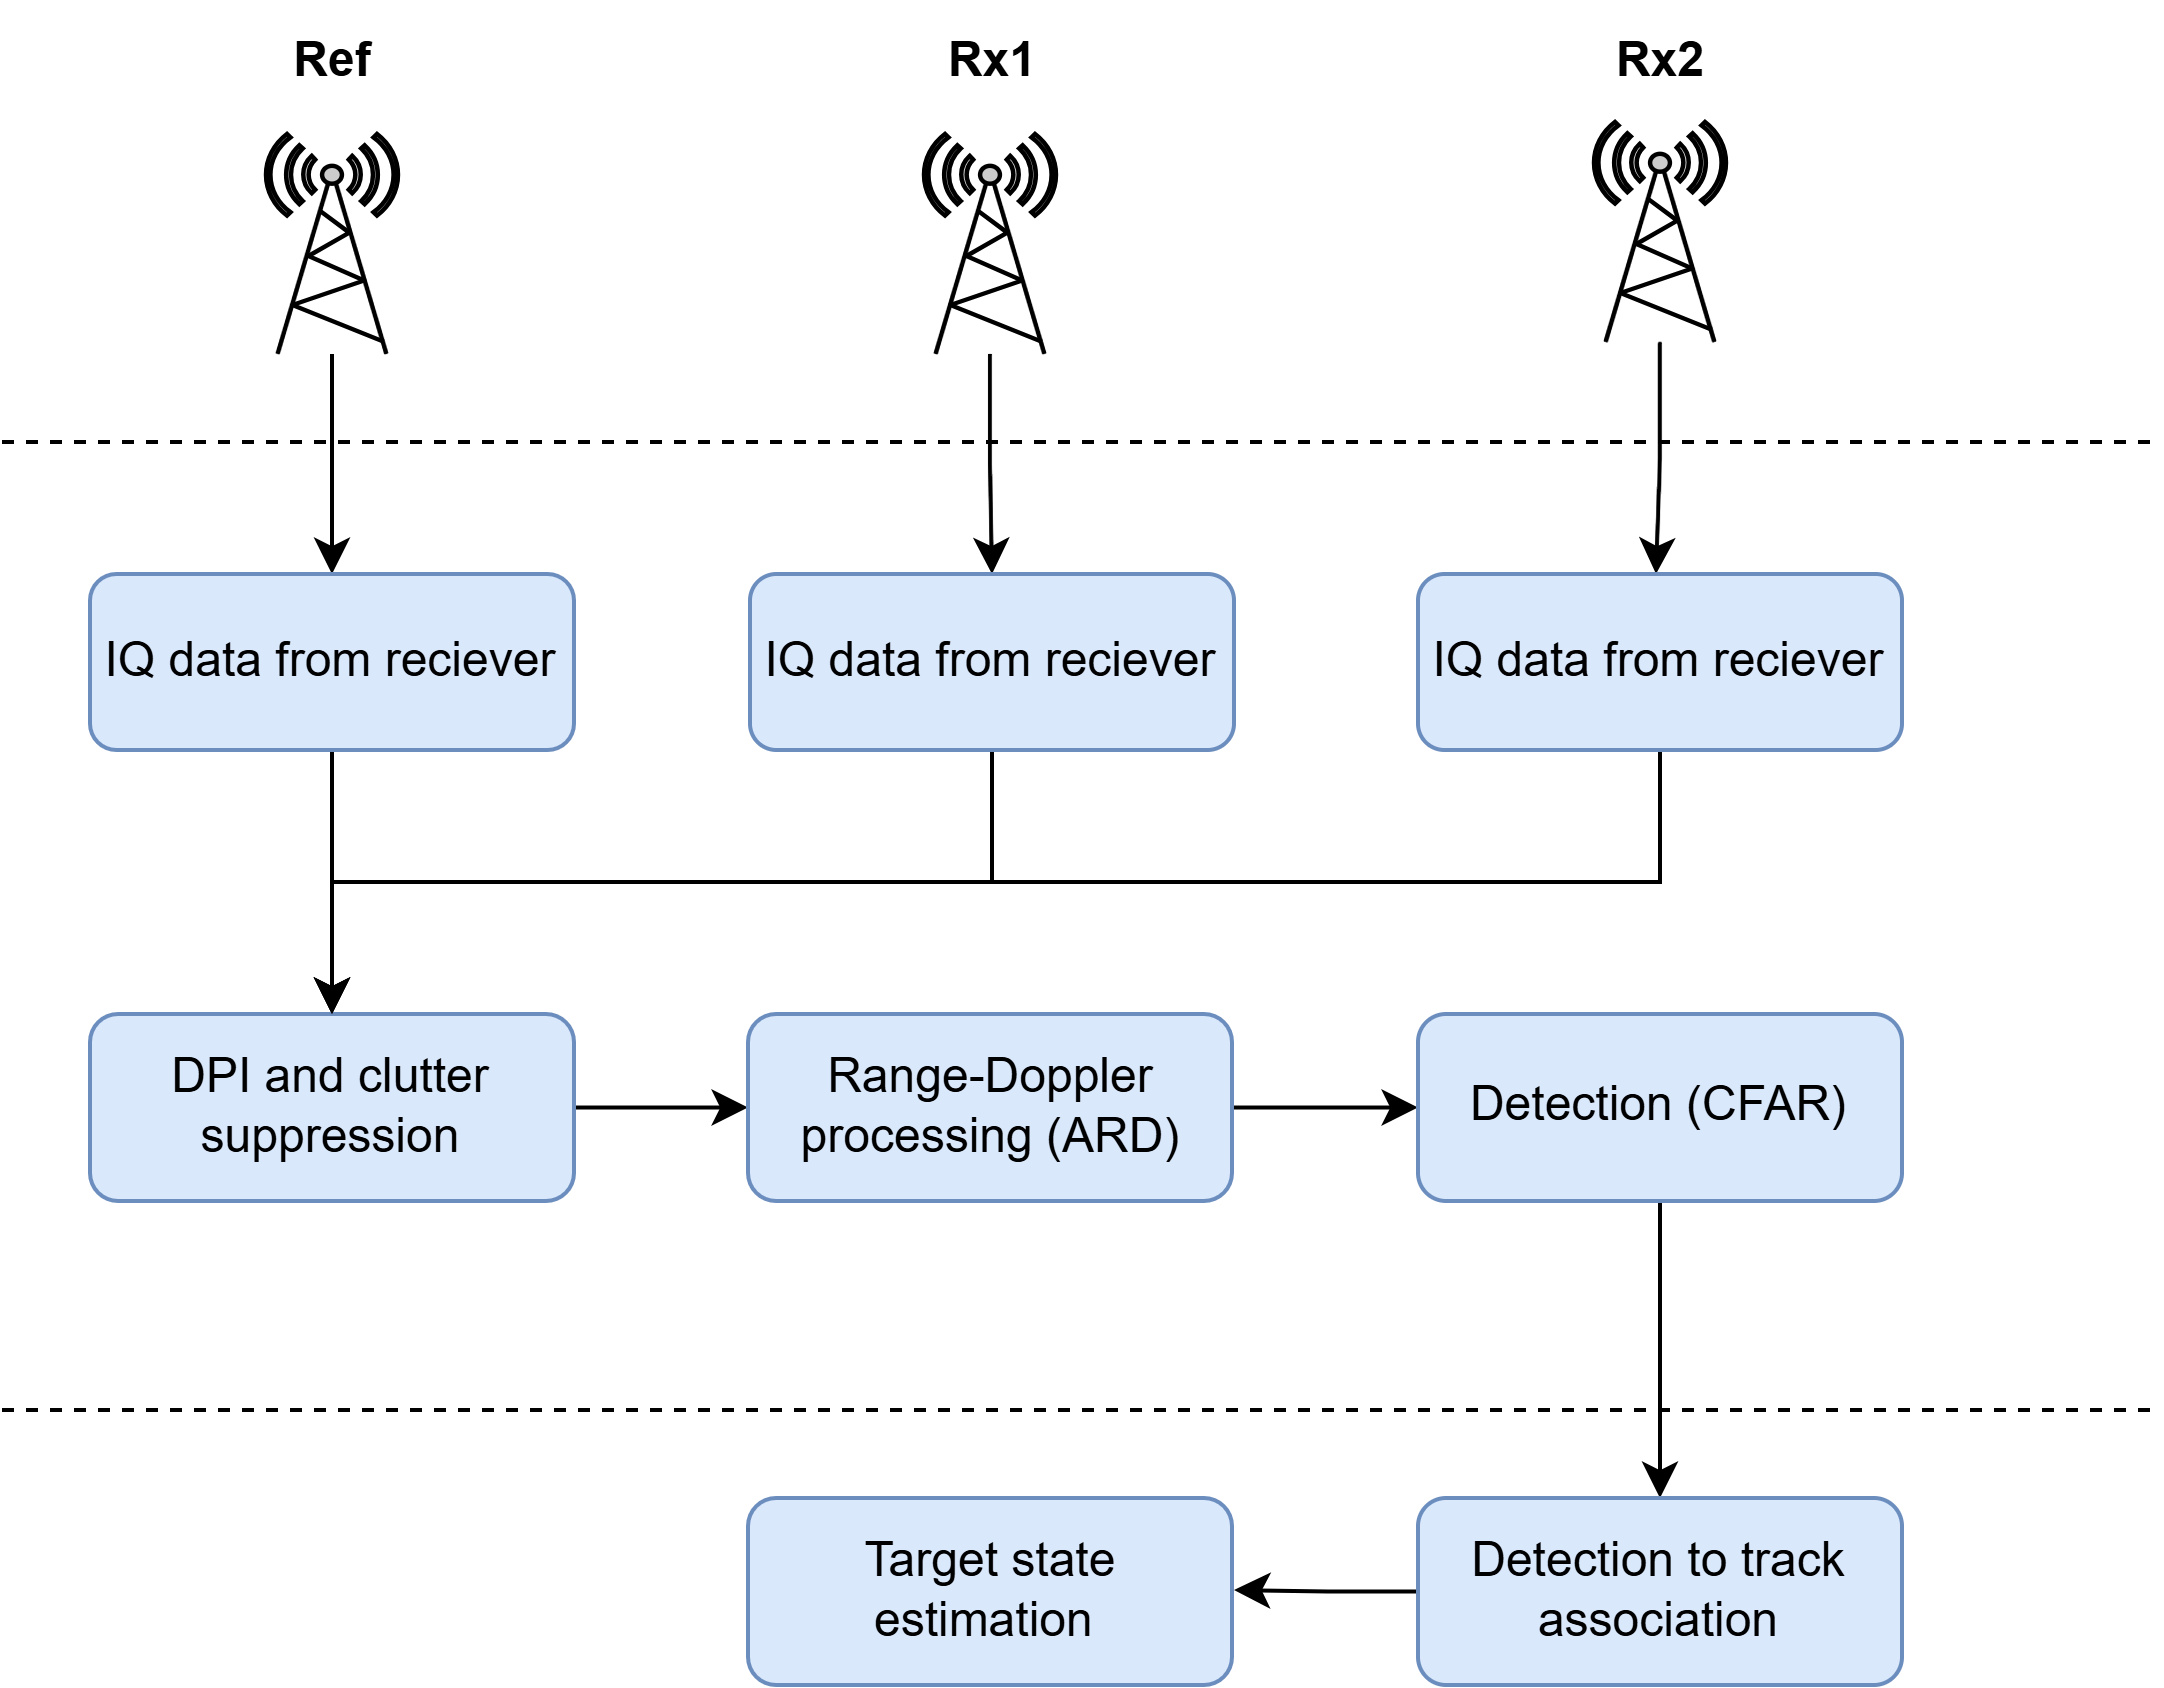
\includegraphics[width=0.9\linewidth]{Figure/fersBistaticRadar.drawio.dsp2.png}
	\caption{Signal Processing Block used for processing signals from the receiving antennas.}
	\label{fig1:spu}
\end{figure}

The general method of evaluating target positions from a bistatic or multi-static \ac{Radar} setup by calculating the difference in range between the target and multiple known locations is known as localization \cite{Friedlander1987}. In \cite{Howland2005a}, the received echo and the reference signal are correlated to compute the relative delay which is related to the bistatic range. The bistatic range is the total distance, measured as the sum of the range from the transmitter to the target and from the target to the receiver. The cross ambiguity function, which represents the correlation between the reference signal and the echo signal as a function of time delay and Doppler frequency shift is then used to calculate the \ac{TDOA} parameters and Doppler shift of the target. The cross ambiguity function \( \chi(\tau, \nu) \) is defined as:
\begin{equation}
\chi(\tau, \nu) = \int_{-\infty}^{\infty} s_T(t) s_R^*(t - \tau) e^{-j2\pi\nu t} \, dt
\label{crossamb}
\end{equation}

where \( s_T(t) \) represents the transmitted (reference) signal, \( s_R(t) \) is the received (echo) signal, \( \tau\) is the time delay, \( \nu \) is the Doppler frequency shift and \( s_R^*(t - \tau) \) is the complex conjugate of the received signal delayed by \( \tau \). Target localization is then achieved by identifying the highest value of correlation on the cross ambiguity function which indicates the time delay and frequency shift where the echo and reference best match \cite{Khalafalla2024}.
%%%% Typical Applications 

\subsection{State Estimation}
%History of state estimation
The history of state estimation dates back to more than 200 years ago when C.F Gauss presented his work on the method of least squares in 1821 and 1823, although Legendre had already investigated it in 1806 followed by Laplace in 1812 who also did an intensive study on problems of estimation\cite{Physics}.
%What is State estimation in Passive \ac{Radar}

The state of a system comprises one or more variables that characterize the status of a system at a given time; for instance, in the case of a moving target like a vehicle, these variables can represent parameters such as position, velocity and acceleration of the target. The problem of state estimation focuses on estimating the state of the system since the true state of the system is typically not directly measurable or known. Instead, observations of the state are made indirectly through measurements which are also affected by noise \cite{Dunik2020}.

In \cite{Levy2008}, the problem of estimation is explored through various methods that differ in design philosophy and metrics used for performance evaluation. This review follows a similar approach, covering the following methods:
\begin{itemize}
    \item Bayesian Estimation methods
    \item Frequentist approach to estimation problems (Classic Estimation)
\end{itemize}
%Bayesian Estimation
In  Bayesian estimation methods, all parameters of the state are treated as random variables, and their probability distribution can be derived either from physical modelling approaches or empirically through extensive data collection from numerous experiments \cite{Levy2008}. The primary objective is to determine the \ac{PDF} of the state $x_k$ given the measurements $z_k$. This \ac{PDF} denoted as $p(x_k \mid z_k)$, represents the conditional probability of the state $x_k$ given the observed measurements $z_k$ where $p(x_k \mid z_k)$ describes the likelihood of the state $x_k$ given the specific measurements $z_k$ \cite{Dunik2020}.

%Frequentist estimation 
In the frequentist approach, all parameters are considered fixed but unknown and are estimated solely based on the observations or measurements. Among such estimators, the \ac{ML} estimator is an optimization approach that determines the values of the unknown parameters that maximize the likelihood of the observed data occurring \cite{Levy2008}. The development of a state estimator relies on a state-space model that represents the physical dynamics of the system \cite{Hasdiana2018}. In the case of a moving object, the model describes the kinematic relationship of the state variables. Additionally, the design of the state estimator also comprises of a measurement model which describes the relationship between the sensory data or measurements and the state of the system. 

In Figure \ref{fig:generic_state_space_model} a generic state space model adapted from \cite{CHEN2} is illustrated to model the stochastic filtering problem. Given the initial density $p(x_o)$, transition density $p(x_t|x_{t-1})$, and likelihood $p(y_t|x_t)$.
The primary goal of filtering is to determine the optimal current state at time $t$ by using all the measurements available up to time $t$ taking into consideration the input data as well. For instance, the Kalman Filter operates as a predictor-corrector algorithm where the predictor models the evolution over time while the corrector updates the estimate based on measurements \cite{Richards2010}.
%State space models
\newline
\begin{figure}[ht!]
	\centering
	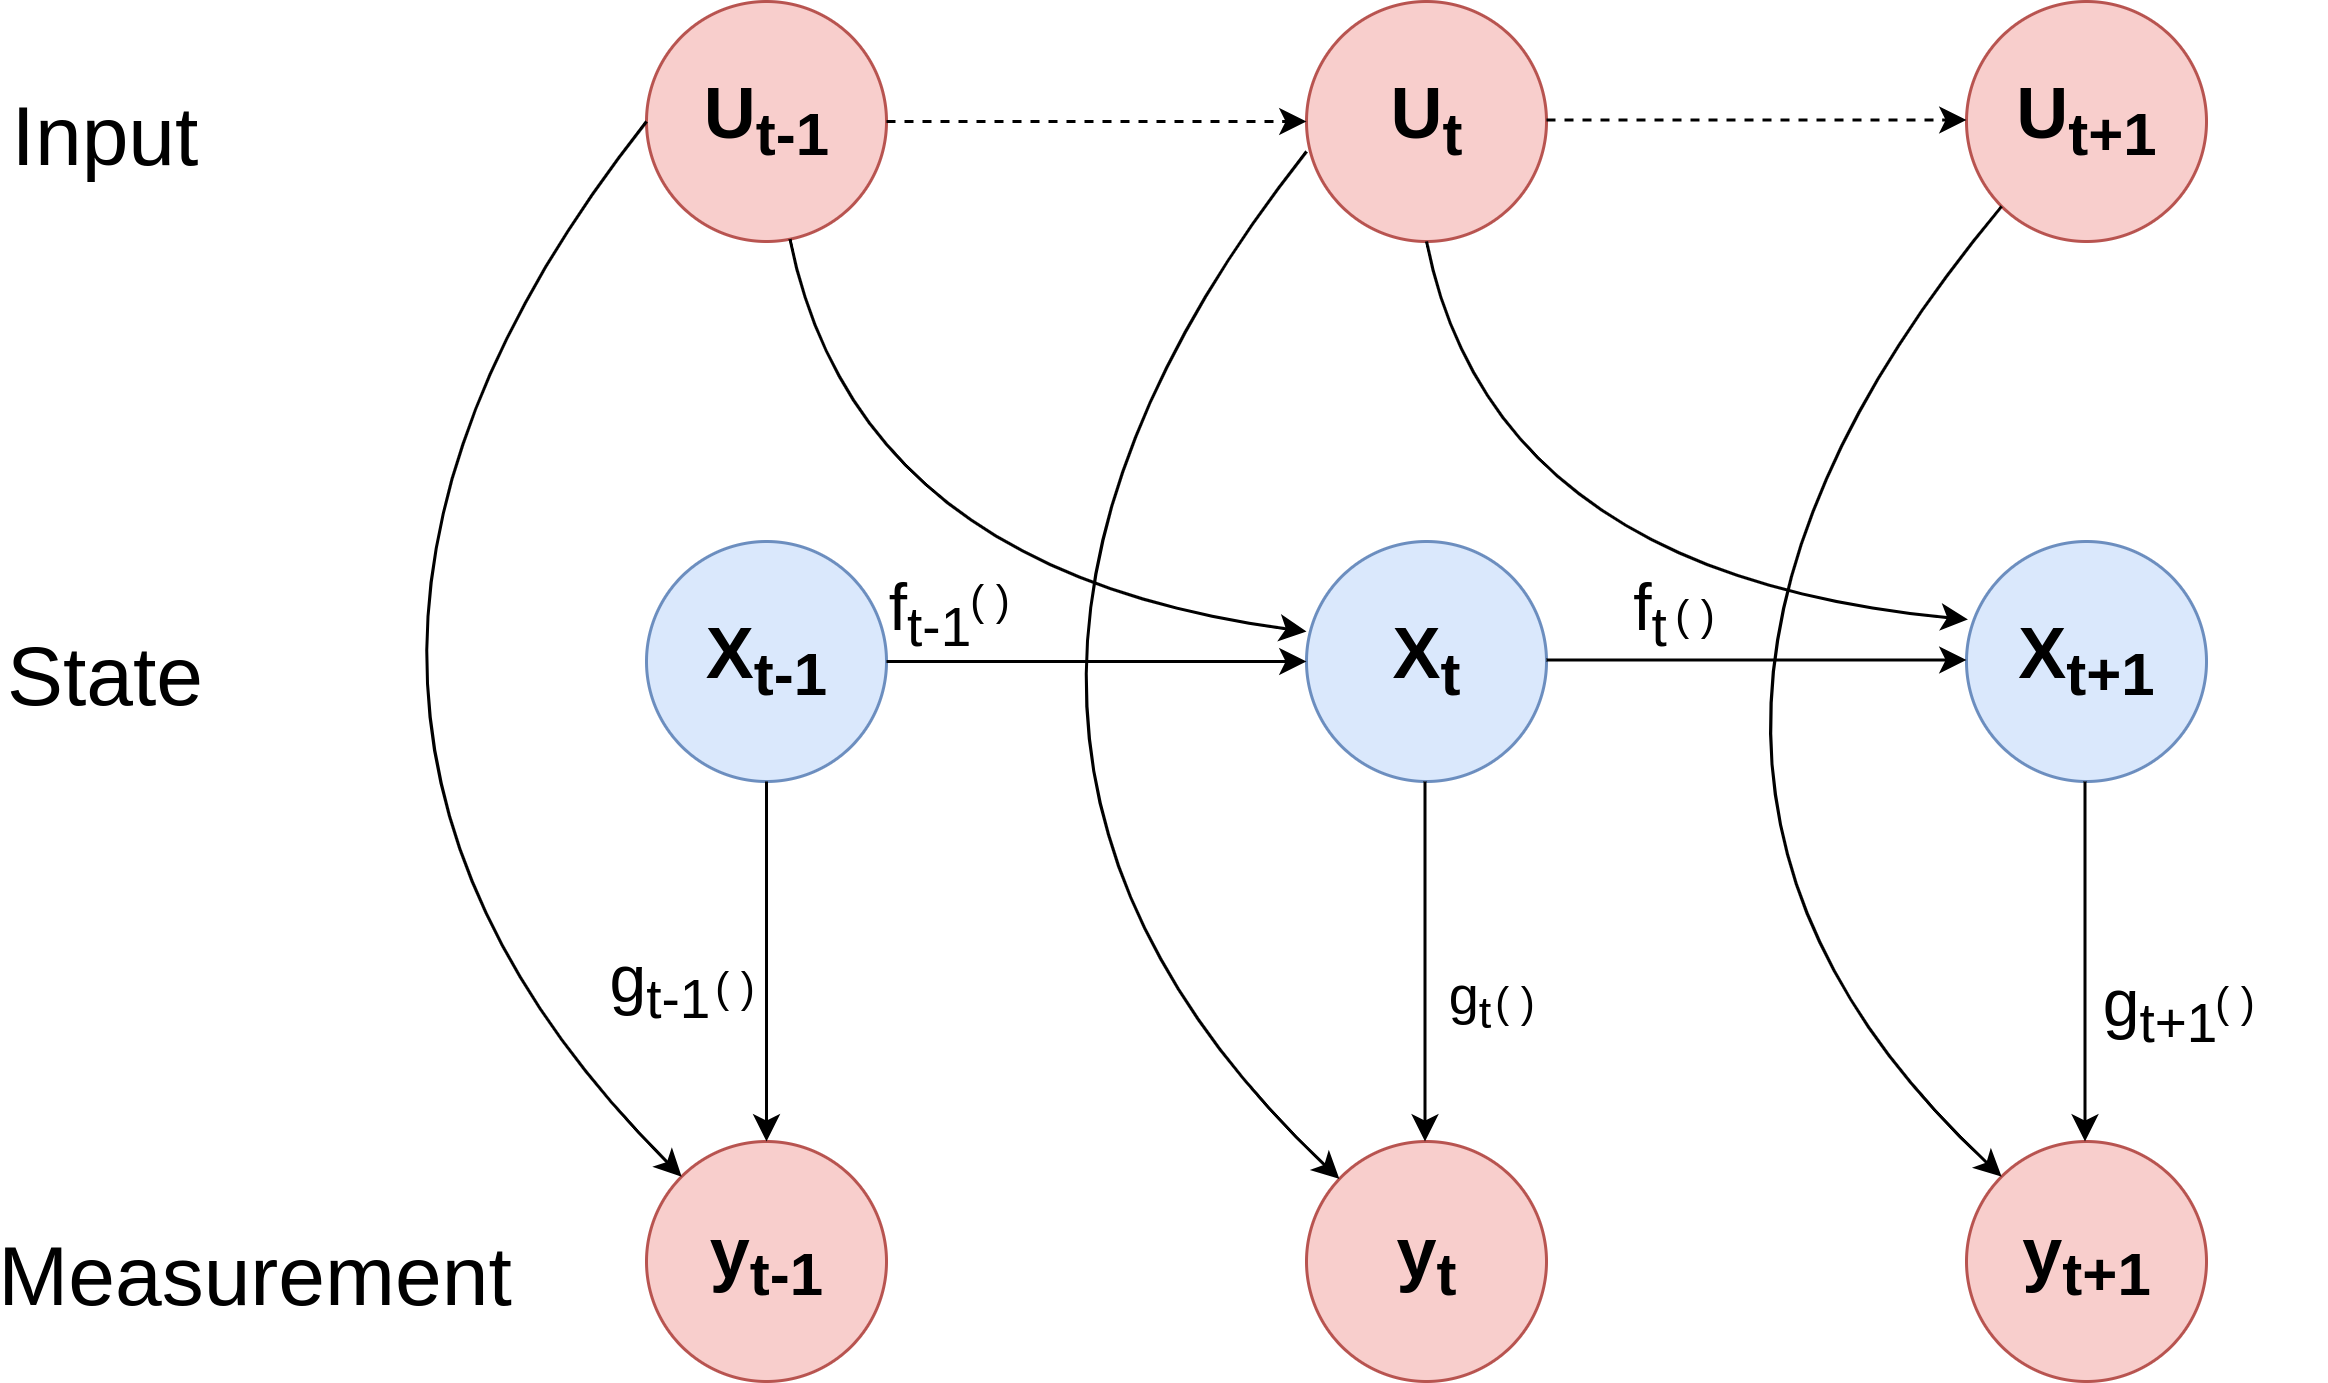
\includegraphics[width=0.75\linewidth]{Figure/genericStateSpace.drawio (1).png}
	\caption{A generic state-space model.}
	\label{fig:generic_state_space_model}
\end{figure}
%Continous vs discrete time

\section{Tracking Filters}
In the introduction, the historical context of \ac{PR} and various estimation methodologies used in estimation theory were explored. This section focuses on tracking filters extensively utilized in \ac{Radar} systems. Specifically, a review of the Kalman Filter and its variants, Particle Filters, Gauss-Newton Filters, Polynomial Filters, and tracking filters based on deep learning is presented.

\subsection{Kalman Filter}
Stochastic filtering emerged in the mid-twentieth century, largely inspired by the groundbreaking contributions of Norbert Wiener, who formulated optimal signal estimation from noisy measurements as a rigorous mathematical optimisation problem. The Wiener filter minimised the mean square error of the estimate using the statistical properties of the signal and noise, and attracted interest among mathematicians, scientists, engineers and computer scientists \cite{CHEN2003}. However, it required the entire measurement history and assumed stationary processes, making it unsuitable for real-time applications, limitations that Kalman would later address through a recursive reformulation of the problem.
%Prior to Kalman's work, Wiener filters required the entire measurement history and assumed stationary processes, making them computationally prohibitive for real-time applications and unsuitable for tracking dynamic targets.In 1960, Rudolf E. Kalman introduced a revolutionary approach that fundamentally changed the landscape of estimation theory \cite{Kalman1960}. The Kalman Filter's key innovation was its \textit{recursive} structure, which required only the previous state estimate and current measurement to compute the optimal estimate—eliminating the need to store or reprocess historical data. This breakthrough enabled real-time implementation on the limited computing resources available in the 1960s.Furthermore, Kalman's state-space formulation allowed the filter to handle \textit{non-stationary} and \textit{time-varying} systems, a critical requirement for tracking maneuvering targets. For linear systems with Gaussian noise, the Kalman Filter is provably optimal in the minimum mean-square error sense, providing both theoretical guarantees and practical performance.
The Kalman Filter and its various adaptations have played a significant role in filter theory for many years. As noted by S. Chen \textit{et al.} \cite{CHEN2}, \textquotedblleft Kalman Filters are widely used in modern engineering and scientific disciplines, including communications, machine learning, neuroscience, economics, finance, and political science, among others\textquotedblright. However of importance to this project, is the use of Kalman Filters in FM \ac{PR}.

%application in Apollo project
The Kalman Filter revolutionized state estimation through its recursive formulation, which enabled real-time computation using only the previous state estimate and current measurement, in contrast to earlier methods like the Wiener filter that required storing and processing entire measurement histories \cite{Andrews2010,schmidt1981}. The Kalman Filter was utilized in the Apollo Project to estimate the spacecraft's position and facilitate complex orbital trajectories. This was particularly crucial for the return journey, where the Apollo Command Module, with its three-member crew, had to re-enter the Earth's atmosphere at an optimal angle. An excessively steep angle would result in the module burning up, while a shallow angle could lead to it bouncing off the atmosphere \cite{Andrews2010}. In 1961, a team led by S.F Schmidt at \ac{NASA} \ac{ARC} implemented the Kalman Filter in digital computer simulations to tackle the circum-lunar navigation challenge and also solved the Apollo guidance and navigation problem using a mainframe computer with a 36-bit floating-point arithmetic \cite{Andrews2010}. This practical implementation demonstrated the filter's capability to handle non-stationary, time-varying dynamics with limited computational resources.

It is well-established that the Kalman Filter has been extensively utilized over the years, spanning from conventional \ac{Radar} tracking domains to now tracking in domains such as Doppler and bistatic range \cite{Joshi2022,Howland2005a}. For instance,  Howland et al.~\cite{Howland2005a}  demonstrated that a four-state Kalman Filter can effectively associate target echoes in the range and Doppler space using FM bistatic \ac{Radar}. Furthermore, in \cite{Joshi2022}, a ship tracking algorithm was proposed which does target tracking in range and Doppler space using range compressed airborne \ac{Radar} data, where a Kalman Filter with \ac{CA} and \ac{CV} motion models are compared to handle target tracking.
%Applications outside \ac{Radar} tracking

Another significant area of research where the Kalman Filter is widely used is visual tracking in computer vision \cite{Gunjal2018, Merven2004}. A method for moving object detection in surveillance systems is demonstrated in \cite{Gunjal2018}, where a target is tracked across video frames by identifying its centre coordinates. The Kalman Filter is used to estimate the location of the moving target from the reference frame to the current frame. Furthermore, N.C. Yang \textit{et al.} \cite{Yang2009} demonstrate the use of Kalman Filtering in video compression to eliminate \textquotedblleft spatial and temporal redundancies in video sequences \textquotedblright. Temporal redundancies are typically addressed through motion compensation techniques, which adjust object displacements from a reference frame to the current frame. In \cite{Yang2009}, a Kalman Filter-based motion estimation algorithm is presented, improving motion estimation in video coding.

%Challenges and Limitations
Although the Kalman Filter is widely recognized for its simplicity, tractability, and robustness \cite{Julier1997a}, it has notable limitations, particularly when dealing with non-linear state dynamics and observation models. Consequently, variants such as the \ac{EKF} and the \ac{UKF} are frequently employed to address these challenges. These variants address the limitations of the standard Kalman Filter, offering better performance in non-linear applications. The variants of the Kalman Filter and other tracking filters are discussed in the subsequent sections of the literature review.

\subsection{Extended Kalman Filter}
The \ac{EKF} is a non-linear adaptation of the Kalman Filter, specifically designed for handling non-linear systems. It follows a similar approach to the Kalman Filter but differs in how it handles the system dynamics. Unlike the standard Kalman Filter, which assumes linear state transition and observation models, the \ac{EKF} extends its applicability to non-linear systems by requiring that these models be differentiable. It achieves this by leveraging the differentiability of the state transition and observation functions, enabling linear approximations through first-order Taylor series expansions\cite{Aditya}. The \ac{EKF} can be viewed as the non-linear version of the Kalman Filter which allows for the linearization of non-linear models about the current estimate. 

For non-linear dynamic systems, the linear Kalman Filter becomes inadequate because it is not possible to define the process or measurement models using the multiplication of vectors and matrices. The \ac{EKF} provides an efficient solution for dealing with non-linear models and has been extensively used in \ac{Radar} for tracking maneuvering targets with non-linear state dynamics. Kim and Bang in \cite{Kim}, also emphasize that the \ac{EKF} is computationally more efficient than other non-linear filtering methods such as point-mass filters and Particle Filters. Furthermore, its widespread use in real-time applications highlights its practical significance where the Kalman Filter falls short.

Key steps for the digital computer simulations at \ac{ARC} for solving the circum-lunar navigation problem led to the development of the \ac{EKF}. Monte-Carlo analyses demonstrated that the non-linearities of the trajectory did not affect the accuracy of the \ac{EKF} for the expected error ranges for the Apollo missions \cite{Andrews2010}. Furthermore, the studies at \ac{ARC} indicated that \ac{EKF} would give comparable accuracies to the weighted least squares estimator while significantly reducing the requirements for onboard computer memory and computation speed \cite{schmidt1981}. However, at that time the \ac{EKF} had not yet been verified to function properly with the available flight computers, a challenge later addressed by the \ac{MIT} laboratory in their subsequent work on the Apollo system.

%Some work done using EKF
Since its initial implementation, the \ac{EKF} has been extensively utilized in applications where the errors from the linear approximations are negligible compared to the measurement errors. A prominent application of the \ac{EKF} is its role in estimating position and velocity in \ac{GNSS} receivers to synchronize the receiver clock with \ac{GPS} \cite{Grewal2006}. Of importance to this research is the application of the \ac{EKF} in \ac{Radar} target tracking, in a study conducted in \cite{Measurements2023b} the \ac{EKF} is implemented to track targets in a \ac{3D} Cartesian space using bistatic range and range rate measurements with a \ac{PBR} system that has no bearing angle information. Furthermore, the \ac{EKF} is demonstrated to be effective in tracking a target using raw measurements of bistatic range and bistatic velocity from a \ac{DVB-T} \ac{PR}, where \ac{EKF}-based tracking is combined with adaptive beamforming techniques for angle estimation \cite{Pasculli2013}.

\subsection{Unscented Kalman Filter}
 The \ac{EKF} as discussed in the previous section, linearizes the non-linear models so that the traditional Kalman Filter can be applied. However, despite the wide usage of the \ac{EKF} as a filtering technique, certain drawbacks such as ease of tuning and implementation in cases where the linearization errors are significant, the filter implementation results in a biased and sub-optimal filter. Recognizing these limitations, Julier and Uhlman developed and demonstrated a novel Unscented Kalman Filter in \cite{Julier1997a} as an improvement over the \ac{EKF} where some of the practical well-known drawbacks of the \ac{EKF} noted in \cite{Julier1997a} are:
\begin{itemize}
    \item \textquotedblleft Linearisation can lead to significant instability in filters if the assumption of local linearity is violated\textquotedblright, as noted by S.J. Julier in \cite{Julier1997a}.
    \item Computing the Jacobian matrices is often complex in many applications, posing major challenges during implementation.
\end{itemize}
In \cite{Julier1997a}, the analytical superiority of the \ac{UKF} over the \ac{EKF} was demonstrated. The \ac{UKF} operates on the principle that a discretely sampled set of points can effectively characterize both the mean and covariance. These sample points accurately represent the true mean and covariance of a Gaussian random variable. As noted by Z. Cai and D. Zhao \cite{Cai2006},  \textquotedblleft When the sample points are passed through the true non-linear system, they effectively capture the updated mean and covariance accurately to the 3rd order (Taylor series expansion) for any non-linear function compared to the 1st order (Taylor series expansion) linearisation in \ac{EKF}\textquotedblright.

The \ac{UKF} uses the unscented transform where deterministic sample points account for non-linearities of the system \cite{Yin2021}. Although the \ac{UKF} achieves the accuracy of a third-order Taylor series expansion, it does so without the computational complexity of calculating the Jacobian matrix. According to A. Asif  \textit{et al.} \cite{Measurements2023b}, \textquotedblleft there is no general formula for calculating the values of the sigma points; therefore, it is crucial to make accurate approximations of the parameters based on the specific estimation problem\textquotedblright.

%Applications of the EKF
In most applications requiring high accuracy state estimation such as autonomous navigation, the \ac{UKF} is usually used over the \ac{EKF} \cite{Costanzi2017,Grewal2006,Costanzi2019}. In \cite{Costanzi2017}, the \ac{UKF} is compared to the \ac{EKF} where the \ac{UKF} is illustrated to be effective in bearing-only target localization even when the positions of the sensors are unknown. In another study \cite{Ortenzi2009}, the \ac{UKF} is compared to the \ac{PF}, showing that the \ac{UKF} offers comparable performance to the \ac{PF} with reduced computational load and ease of algorithm setup in a bistatic \ac{Radar} environment where a non-cooperative \ac{FM} radio station is used as a transmitter of opportunity.
%limitations of the UKF

Similar to the \ac{EKF}, the \ac{UKF} is limited to models with Gaussian noise assumptions \cite{Konatowski2017}. For state estimation in scenarios where models do not adhere to Gaussian assumptions or involve non-Gaussian noise, Particle Filters offer a viable alternative. In the next section, a review of the literature on Particle Filters is presented.
%Gaussian assumptions
%
\subsection{Particle Filters}
The Particle Filter is a type of sequential Monte Carlo method developed initially for target tracking by N.J. Gordon \textit{et al.}  \cite{NJGordon}. In contrast to the Kalman Filter and its variants (\ac{EKF},\ac{UKF}), the \ac{PF} as highlighted by \cite{MFeroz} operates without the strict assumptions of linearity and Gaussianity. This flexibility allows the \ac{PF} to effectively handle non-Gaussian noise distributions and accommodate non-linearities in both the measurements and dynamics of the target.

Monte Carlo methods use repeated random sampling to generate their results. They begin by defining a domain of possible inputs and then generate random input samples from a posterior distribution over this domain. These samples are used to perform computations, producing output samples, which are then analyzed to infer the output probability distribution \cite{Hoffman}. There are various versions of the \ac{PF} throughout literature, in \cite{Hoffman} different state-space Particle Filters based on different resampling methods are discussed namely:
\begin{itemize}
    \item Bootstrap \ac{PF}
    \item Auxillary \ac{PF}
    \item \ac{MCMC} \ac{PF}
    \item Linearised \ac{PF}s
\end{itemize}
In \cite{Arulampalam2007} variants of the \ac{PF} are introduced within the generic framework of the \ac{SIS} and these variants are compared, with some showing better performance in specific applications. Alternative architectures to the generic \ac{PF}s are also proposed for \ac{PR} target tracking \cite{Zhao2013,Tobias2008}.

The superiority of the \ac{PF} over the non-linear Kalman Filters is demonstrated in certain cases. For example, \cite{Abdoul-Moaty2014} shows that the \ac{PF} is more effective as a predictor in a multi-static \ac{Radar} environment, where it successfully corrects its path despite noisy measurements. Additionally, an improvement to the \ac{PHD}-based \ac{PF} for target detection in \ac{PR} is introduced in \cite{Tobias2008}, which enhances reliability and significantly reduces the number of particles required for tracking.

\ac{PF}s have limitations, including their dependence on sample size. A small particle set may not accurately approximate the true state and increasing the sample size, while addressing this issue, also raises computational requirements \cite{Zhong2016}. Particle degeneracy, where many particles have negligible weights, further complicates the situation and is typically addressed through resampling methods. New algorithms proposed in \cite{Zhong2016} tackle particle impoverishment and sampling dependency, resulting in improved tracking performance for non-linear single-variable estimation problems.

In the next section, the Gauss-Newton filters are reviewed, which are also applicable to non-linear dynamics and observation models.

\subsection{Gauss Newton Filter}
%What are Gauss-Newton Filters
Gauss invented the method of least squares and the Gaussian \ac{PDF} at the beginning of the nineteenth century \cite{Zhichao2018}. This was a significant breakthrough in estimation theory. By combining this with the differential calculus developed by Newton, Gauss created the Gauss-Newton algorithm.
%Limitations and Disadvantages
In 1958, Swerling \cite{Zhichao2018} found that the non-recursive Gauss-Newton algorithm was unsuitable for tracking targets such as satellites due to the limited computational capacity of computers at that time. He proposed a new recursive algorithm later known as the Swerling filter. With today's vast processing capacities, the Gauss-Newton filter has become feasible for application in some non-linear systems.

The Gauss-Newton filter allows for long prediction times, enabling data updates without intervals. Its finite memory length can be varied, which allows for adaptability, making it suitable for estimating targets with high dynamics. In this case, the filter acts like a sliding window, focusing on the most recent 
observations \cite{nmorris2013}. 

\begin{comment}
        
Table \ref{gnf_key_attributes} adapted from \cite{improvedGauss} highlights some of the key attributes of the Gauss-Newton filters compared to the linear Kalman Filter.
\newline
\begin{table}[ht]
    \centering
    \renewcommand{\arraystretch}{1.3} % Adjust the row height
    \begin{tabular}{|p{6cm}|p{3cm}|p{3cm}|} % Adjust column widths
    \hline
    \textbf{Key Attributes}                 & \textbf{GNF}   & \textbf{Kalman Filter} \\ \hline
    Data update frequency                      & flexible timestamps & Constant interval      \\ \hline
    Suitable for highly changing dynamics & Yes            & No                     \\ \hline
    Requires prior initialization                          & No             & Yes                    \\ \hline
    Handles noise in tracking    & Yes            & Yes                    \\ \hline
    Recursive computation                   & No             & Yes                    \\ \hline
    \end{tabular}
    \caption{Key differences between Gauss-Newton Filters and Kalman Filters.}
    \label{gnf_key_attributes}
\end{table}
\newline
\end{comment}


While Gauss-Newton filters provide superior numerical results, robustness, and effectiveness in tracking maneuvering targets, \cite{nmorris2013} highlights that they can suffer from slow convergence or, in some cases, fail to converge. This has necessitated research into enhancements for this filter. Some advancements to the Gauss-Newton filter include merging the \ac{LMA} into the Gauss-Newton filter. In \cite{roaldje}, the iterative version of the Gauss-Newton filter with memory introduced by Norman Morrison in \cite{NmorrisHIll} is adapted to the \ac{LMA} to ensure consistent convergence. It is further demonstrated that the adapted algorithm is robust to random disturbances and non-linear trajectories, where it is used to track targets in Cartesian coordinates with bearing, Doppler, range, and elevation observations \cite{roaldje}. In another study \cite{Morrison}, the Gauss-Newton filter was shown to be able to track aircraft using bearing and Doppler information from a \ac{PR} system.
%Introduce RGNF 

The \ac{GNF}, while robust and effective, it demands substantial computational resources \cite{improvedGauss}. In \cite{costa}, two hardware designs on \ac{FPGA} co-processors are implemented to enhance the performance of the \ac{GNF}. The recursive form of the \ac{GNF}, namely the \ac{RGNF}, was presented to reduce the amount of computational memory required, which was previously recognized as a major limitation for the \ac{GNF} \cite{Inggs1}.

\subsection{Recursive Gauss-Newton Filter}
The Recursive Gauss Newton Filter(RGNF) is an extension to the \ac{GNF}, recently reorganised into a recursive format to track targets in a computationally efficient manner. In \cite{improvedGauss}, the recursive form of the \ac{GNF} is obtained with zero memory to demonstrate the application of the compact recursive form of the \ac{GNF} to non-linear process dynamics and non-linear observation schemes. Subsequent development of the \ac{RGNF} by Nadjiasngar \cite{Inggs1} involves adapting the filter to the \ac{LMA} method similarly to the study in \cite{roaldje} for the \ac{GNF}.
%Some of the applications of the RGNF

The \ac{RGNF} is chosen for tracking targets in a multi-static \ac{Radar} environment that exploits FM radio signals using Doppler-only measurements \cite{De2015}. This study demonstrated the filter's effectiveness in tracking targets with real measurement data collected from at least three receiver sites. Another study \cite{Boyer2012} showed that the \ac{RGNF} significantly outperforms the Kalman Filter and \ac{PF}, resulting in better tracking accuracy and lower computational load for scenarios where the state transition and observation models are linear for tracking in the Doppler and range domain.

\subsection{Polynomial Filters}
Polynomial filters function by fitting a polynomial to a sequence of noisy observations using the least squares method, as introduced in Morrison's book "Introduction to Sequential Smoothing and Prediction" \cite{NmorrisHIll}. These filters are based on Laguerre and Legendre polynomials. Filters based on Legendre polynomials, which have a uniform weight function, are known as \ac{EMP} filters. In contrast, filters based on Laguerre polynomials, which have an exponentially decaying weight function, are called \ac{FMP} filters. The basic structures of the one-step predictor \ac{FMP} and \ac{EMP} filters are similar, allowing for easy switching between the two by changing the weights, this adaptability gives birth to the Composite EMP/FMP filter, which utilizes both types of filters \cite{nmorris2013}.
\newline
\newline
\begin{figure}[ht!]
	\centering
	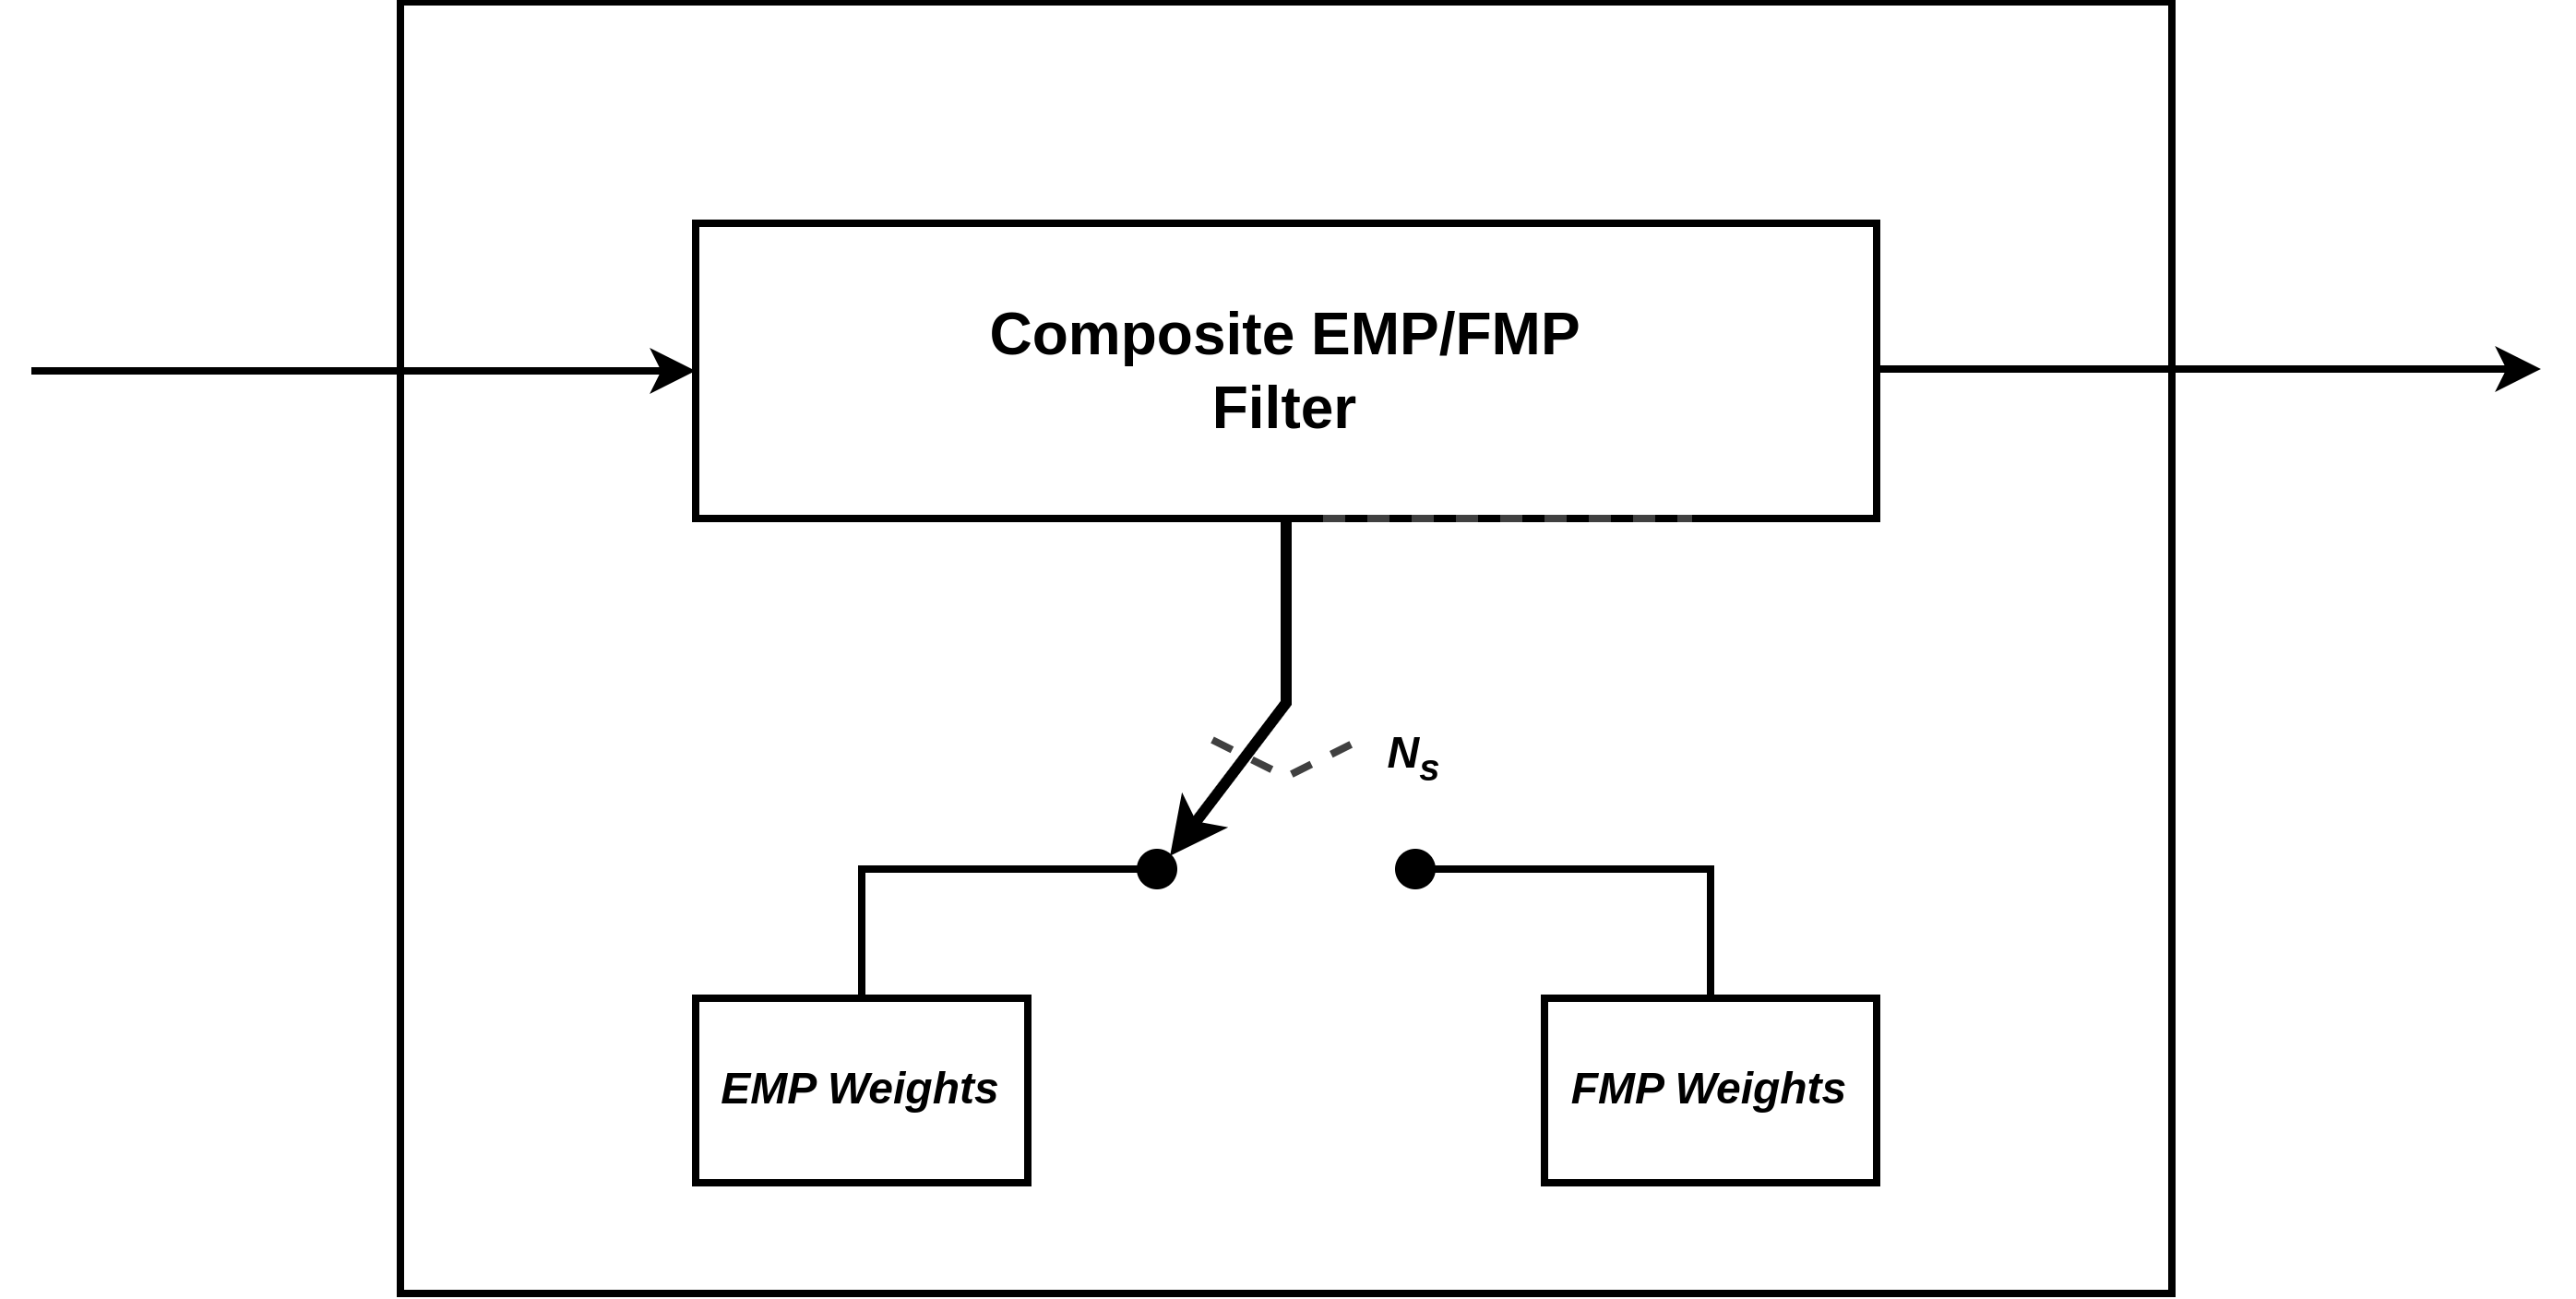
\includegraphics[width=0.85\linewidth]{Figure/compositeP (1).png}
	\caption{Composite EMP/FMP filter.}
	\label{fig:compositeEMP}
\end{figure}
\newline
The Composite Polynomial Filter leverages both the advantages and disadvantages of the \ac{EMP} and \ac{FMP} filters. The \ac{EMP} filter initiates itself automatically but is limited in tracking targets for prolonged periods and can track changing trajectories effectively, whereas the \ac{FMP} filter requires an external initialization but can track targets for longer durations \cite{Boyer2012}. In the Composite filter, as observed in Figure \ref{fig:compositeEMP} adapted from \cite{nmorris2013}, the weights are switched when the filter covariance matrices are equal, which occurs at a transitional sample number  \(N_s\) \cite{nmorris2013}.
\newline 
\newline
According to Norman Morrison's book on Gauss-Newton and Polynomial Filters \cite{nmorris2013}, the composite \ac{EMP}/\ac{FMP} filters, as well as the individual \ac{EMP} and \ac{FMP} filters, can be used for a variety of applications, including but not limited to:
\begin{itemize}
    \item The composite \ac{EMP}/\ac{FMP} filter can be used as a high-data-rate tracker for pedestal control in \ac{Radar} systems and can also be used as a pre-filter for Gauss-Newton or Kalman Filters.
    \item As described in \cite{nmorris2013}, \textquotedblleft the current-estimate \ac{EMP} filter can function as a self-initializing algorithm to initialize Gauss-Newton or Kalman Filters\textquotedblright.
    \item The \ac{EMP} filter can be used to fit a polynomial curve to a sequence of noisy observations using the method of least squares.
\end{itemize}
There are a few studies based on using the composite \ac{EMP}/\ac{FMP} filter for target tracking purposes \cite{Lu2020, Nadjiasngar2011a}. A study in \cite{Lusilao-Zodi2010} \textquotedblleft focuses on the estimation of round-trip time for the transport layer in \ac{TCP} for multimedia applications\textquotedblright. In this study, the filter is used to predict future round-trip times from previously recorded values, demonstrating that the filter can effectively capture model dynamics and non-linearities with less memory space and fast execution times. The composite \ac{EMP}/\ac{FMP} filter is shown to be effective as a pre-filter to the \ac{UKF} for tracking a maneuvering target in a complex scenario \cite{Lu2020}. Furthermore, in \cite{Nadjiasngar2011a}, a \ac{PDA} filter based on the composite \ac{EMP}/\ac{FMP} filter is proposed, achieving comparable results to the Kalman Filter. 

Recent advancements in deep learning have paved the way for new approaches to tracking filters, and in the next segment, a review of some of these methods will be presented.


\subsection{Deep Learning - Based Tracking Filters}
Current filters can generally address the filtering problem for tracking targets. However, as noted by Cui \textit{et al.} \cite{cui2022}, there are still several challenges, such as an excessive number of filtering variants and forms, and a lack of tight coupling with the target motion model. In recent years, there has been a significant trend towards the use of deep learning approaches for target tracking, especially in visual tracking applications \cite{Yang2017,Supreeth2018,Bouzenada2007}. For this review, tracking filters not based on \ac{NN} will be referred to as traditional filters.
\newline
\newline
%What are Neural Networks and categories for Tracking
Throughout the literature, \ac{NN}s are employed in target tracking filters in several distinct ways, as highlighted in  \cite{cui2022}. Some common trends in research for target tracking with \ac{NN}s include: Firstly, integrating \ac{NN}s with traditional filters without altering their structure to enhance performance \cite{Duh2004}; Secondly, using \ac{NN}s to replace specific modules and estimate parameters within traditional filters without changing their overall frameworks \cite{Xu2023}; And lastly, using \ac{NN}s to completely remodel the filtering function, thereby breaking away from the traditional filter's composition and framework \cite{cui2022}. \ac{NN}s are machine-learning models designed to mimic the functionality of biological neural networks in the brain. In terms of computational graphs, traditional filters primarily use linear operations such as division, subtraction, addition, and multiplication, along with nonlinear operations and delayed feedback structures, all of which can be implemented within neural network architectures \cite{cui2022}.
%Network Topologies-
%Some work using neural networks

In \cite{cui2022}, various \ac{NN} topologies are implemented to create a unified model that mimics the operations of both the Kalman Filter and the $\alpha-\beta$ filter. This unified model utilizes \ac{RNN}, \ac{FNN}, and attention mechanisms. The study demonstrates that the non-linear operations of the Kalman Filter can be represented using a \ac{FNN}, where the delayed feedback can be modelled as an \ac{RNN}, and the filter gain can be captured by attention mechanisms.

In another study, a Deep Neural Network-based tracking filter is developed for tracking maneuvering targets  \cite{Liu2019}. This model is trained offline using abundant trajectory data from existing maneuvering targets and has demonstrated superior performance compared to state-of-the-art algorithms for maneuvering target tracking. Furthermore, in \cite{Xu2023}, a Generalized Regression Neural Network (GRNN) is combined with a Kalman Filter to investigate its effectiveness in non-linear approximation from target measurements to target positions. This study highlights the potential of integrating \ac{NN} techniques with traditional filtering methods to enhance tracking performance.

%\subsection{Adaptive Tracking Filters}

\section{Multi-Target Tracking}
In the previous section, various tracking filters used in \ac{Radar} applications were reviewed and were shown to be fundamental for estimating the state of a single target. However, it is essential to examine how these filters fit into the more complex scenario of \ac{MTT}. \ac{MTT} focuses on developing algorithms and techniques for tracking multiple targets simultaneously within an environment under observation. In \ac{Radar} target tracking, \ac{MTT} aims to jointly estimate the number of targets, their states, or trajectories from noisy measurements \cite{Vo2015}. \ac{MTT} involves techniques such as observation to track association and track maintenance.

%\subsection{Target Tracking}
\subsection{Data Association Techniques}
The initial step in multi-target tracking is to accurately interpret sensor data, ensuring that each measured data point corresponds to the correct tracked object. This process typically involves gating and assignment techniques. Several widely used techniques for associating observations with existing tracks are reviewed.
\newline
\newline
\begin{figure}[htb!]
	\centering
    \includesvg[width=1\linewidth]{Figure/MTTDiagram.drawio.svg}
	\caption{Basic elements of a conventional MTT.}
	\label{fig:MTT_Diagram}
\end{figure}
\newline
Figure \ref{fig:MTT_Diagram} illustrates the typical process of updating a track at each update, as described in \cite{Blackman}. The highlighted observation-to-track association block is unique to \ac{MTT}, addressing the combinatorial assignment of M measurements to N tracks. The observation-to-track association technique focuses on the assignment of observations to tracks. Gating, defined as the process of eliminating observations that are unlikely to belong to a track based on a specific gating method, reduces computation for the data association step \cite{Konstantinova2003}. Data association illustrated as observation-to-track association in Figure \ref{fig:MTT_Diagram}, occurs after the gating process. This step is crucial for densely spaced targets, where additional logic is needed to determine the most likely target for each track.

In an environment with clutter, some of the measurements being fed into the tracker may not be due to real targets but rather to clutter or false alarms. This causes ambiguities in associating the existing target tracks with the measurements at every update. Such ambiguities can result in poor target tracking and overwhelm computational resources. As a result, there has been extensive research in the area of \ac{MTT} to resolve the problem \cite{Blackman}. One of the most used methods of data association in \ac{MTT} is the \ac{GNN} approach \cite{Liu2022,Shi2013,Konstantinova2003}.

\subsubsection{Global Nearest Neighbor}
The \ac{GNN} is an extension of the Nearest Neighbor association that functions by searching for unique joint associations of measurements from targets to tracks, maximizing likelihood or minimizing distance \cite{Stevens2011}. One of the advantages of the \ac{GNN} is its simplicity in implementation, as well as its low memory and computational resource usage because it only uses the most likely hypothesis for data association \cite{Shi2013}. A modified version of the \ac{GNN} is used to perform data associations in the presence of sensor bias based on the relative distance or topology of the sensor observations \cite{Shi2013}. A study in \cite{Saputra2023} utilizes the \ac{GNN} as a \ac{MTT} due to its fast execution time for application in aircraft tracking for Ground-Controlled Interception \ac{Radar}. In another study, the \ac{GNN} is used to effectively associate inter-frame detections from a Video Synthetic Aperture \ac{Radar} image sequence. The \ac{GNN} filter is prominent in the space of \ac{MTT}; however, there are certain drawbacks to it despite its efficiency. In \cite{Smith2019}, it is noted that it is prone to losing tracks and having poor performance in cases where targets are closely spaced. Misassignment or track loss can be severe for the filtering process, causing the filter to slowly converge or fail to converge.

\subsubsection{Joint Probabilistic Data Association }
%% Probability data Assoiication filter
The \ac{JPDA} is derived from the \ac{PDA}, which was introduced in the 1970s \cite{Bar-Shalom1974}. Unlike the \ac{PDA}, which considers each measurement-target association independently, the \ac{JPDA} computes the association probabilities jointly across all targets. This means that at each update, the \ac{JPDA} uses all measurements and weighs them according to their respective association probabilities \cite{OnderBozdogan2016a}. It is also mentioned in \cite{Blackman}, that the \ac{JPDA}  outperforms the \ac{GNN} in heavily cluttered multi-target environments. For this reason, the \ac{JPDA} algorithm is widely used in \ac{MTT} research. In \cite{Khalil2016} it is demonstrated that the \ac{JPDA} used in conjunction with the Constant Turn Rate Model \ac{UKF} can provide accurate state estimates of a target while minimizing track loss. The study in \cite{Braca2012}, shows the usage of \ac{JPDA} and \ac{UKF} applied to target tracks generated by two \ac{HFSW} \ac{Radar}s and \ac{AIS} data. Despite the widespread adoption of the \ac{JPDA}, the \ac{JPDA} has limitations due to its combinatorial nature, requiring substantial computational resources. To address this problem \ac{RFS} methods are usually implemented.

\subsubsection{Random Finite Set Methods}
As previously discussed, an \ac{MTT} scenario involves a collection of individual target states and measurements, in contrast to single target systems, where the state and measurement of the target at time \( k \) are two vectors with possibly different dimensions. These multi-target states and measurements can vary over time as targets appear and disappear. An \ac{RFS} is a set of finite-set-valued random variables and consists of a random number of points \cite{Jerrelind2020}. An \ac{RFS} instance \( X = \{x_1, \ldots, x_n\} \) consists of random, distinct, and unordered points, making \ac{RFS} a natural representation for multi-target states and measurements \cite{Vo2005}. In \cite{Jerrelind2020}, the \ac{MTT} problem is formulated as a filtering problem with a multi-target state space \( \mathcal{F}(\mathcal{X}) \) and observation space \( \mathcal{F}(\mathcal{Y}) \), where the sets of targets and measurements are denoted as \( X_k \) and \( Y_k \) respectively \cite{Jerrelind2020}.
\newline
\begin{equation}
    X_k = \{ x_{k,1}, \ldots, x_{k,M_k} \} \in \mathcal{F}(\mathcal{X}) 
\end{equation}
\begin{equation}
    Y_k = \{ y_{k,1}, \ldots, y_{k,N_k} \} \in \mathcal{F}(\mathcal{Y}) 
\end{equation}
\newline
Here, \( M_k \) represents the number of targets and \( N_k \) denotes the number of measurements at time \( k \). Among the various methods based on the \ac{RFS} framework is the \ac{PHD} filter \cite{Clark2005,PHAMNAMTRUNG2007,Vo2005}. The \ac{PHD} filter is an algorithm for \ac{MTT} that recursively estimates both the number and states of multiple targets based on a set of observations \cite{Prihoda2019}. Between 1993 and 1995, in several unpublished manuscripts, Stein \textit{et al.} introduced the concept of \ac{PHS}. This concept involves a probability distribution graph that, when integrated over a target space region, yields the expected number of targets within that region \cite{Mahler2000}. This idea laid the groundwork for the \ac{PHD} filter, which represents the expected value of a random track set and, when integrated over a state space region, determines the precise random number of targets in that region.

A study in \cite{Guldogan2014} addresses the problem of \ac{MTT} in a bistatic \ac{Radar} setup from sensors measuring the Doppler shift. The \ac{PHD} filter and two of its variants are also compared: the \ac{GM-PHD}, introduced in \cite{Vo2006}, which assumes targets follow a linear Gaussian dynamical model with linear Gaussian measurements, and where survival and detection probabilities are state-independent; and the \ac{SMC-PHD}, proposed in \cite{Vo2005}, which offers a more flexible approach compared to the Gaussian Mixture \ac{PHD}, accommodating a broader range of scenarios. It was found that both variants can track multiple targets successfully using Doppler measurements only, with the \ac{GM-PHD} being more effective and easier to implement than the \ac{SMC-PHD}. 

Another variant of the \ac{PHD}, the \ac{CPHD}, is explored in \cite{Ozkan2011} for tracking multiple ground vehicles using acoustic sensor arrays, where the \ac{CPHD} is shown to perform better than the \ac{PHD}. While \ac{RFS} methods are effective for addressing \ac{MTT} problems, the \ac{PHD} filter has a major drawback in terms of computational efficiency \cite{Prihoda2019}, however the \ac{PHD} variants have proven to be robust and more efficient in addressing these issues. Another advantage of \ac{PHD} filters is that they model the birth and death of targets in the observation space, where other data association techniques such as \ac{GNN} and \ac{JPDA} require additional logic for managing the trajectories of targets during the tracking process. Various methods of track management are discussed in the track management section of the review.

\subsection{Track Management}
Track management, also known as track maintenance, is a critical component of the target tracking process. It involves several key functions:
\begin{itemize}
    \item \textbf{Track Initiation}:
    \newline
    This involves assigning a detection to a new track when it is not associated with an existing track. Once a track is initiated, it is considered tentative until further validation.
    
    \item \textbf{Track Confirmation}:
    \newline
    This process verifies the validity of a detected target. It typically involves logic for determining the status of the track based on additional observations.
    
    \item \textbf{Track Deletion}:
    \newline
    This involves removing a track when it is no longer deemed valid. A track may be deleted if the target is lost if it is determined to be a false alarm, or if it has not been updated within a specified time frame.
\end{itemize}
One common approach in track management is the M-out-of-N logic, which is valued for its simplicity \cite{Boyer2012, Kim}. According to this logic, a track is confirmed if there are \(M\) validated detections out of the last \(N\) samples. Conversely, a track is terminated if there have been no valid detections for \(M\) out of the last \(N\) samples. Additionally, unassociated measurements can be used to create new tracks \cite{Braca2012}. For instance, in \cite{Kim2013}, the M-out-of-N logic was applied to a multiple target tracking problem for a \ac{FMCW} \ac{Radar}. This method was used to evaluate the quality of both confirmed and tentative tracks, ensuring that tracks with a low probability of loss were maintained even in the presence of clutter.

Other track management techniques include methods based on track score tests, such as the \ac{SPRT}, Bayesian sequential tests, and batch processing techniques \cite{Blanding2009, Blackman}. \ac{SPRT}-based methods create tentative tracks from detections that are not initially correlated with existing targets. These tracks remain provisional until a sufficient number of observations have been collected to make a statistically reliable judgement. The decision to confirm or terminate a track is based on comparing the likelihood of observations under two hypotheses: a true target hypothesis versus a false alarm hypothesis \cite{Blanding2009, Kajenski2011}. A track is confirmed if its score meets or exceeds a specified threshold; otherwise, it is terminated if the score falls below this threshold.

Bayesian sequential tests, similar to \ac{SPRT}, use Bayesian methods to recursively update the posterior probabilities of various hypotheses. Batch techniques, such as the Hough Transform \cite{Leung1996}, process detections over multiple frames collectively \cite{Blanding2009}. The Hough Transform has been shown to offer long track lifetimes, low false data association rates, and short computational times \cite{Leung1996}.

Despite advancements in track management techniques, the M-out-of-N method remains popular for its simplicity and efficiency. Additionally, in \cite{Khalil2016a} combining the M-out-of-N technique with \ac{JPDA} has been shown to provide accurate estimates of target positions and velocities in automotive \ac{Radar} applications.

\section{Performance Evaluation of Tracking Filters }
In the preceding subsections, various tracking filter algorithms and techniques used in \ac{MTT} have been reviewed. Evaluating the performance of these tracking algorithms is also crucial to determine their efficiency, robustness, and accuracy. When ground truth data is available, metrics such as \ac{RMSE} and \ac{NEES} are frequently used to evaluate the accuracy of the tacking filter estimations through Monte Carlo simulations \cite{Ding, Omar2012a, Inggs1, Nadjiasngar2011a}. Additionally, the Cramér-Rao Lower Bound (CRLB) and its variants, including the \ac{PCRLB} and the \ac{CCRLB}, are also commonly employed performance measures \cite{Junler2020, Nadjiasngar2012, Bauermeister2016}. However, there has been limited research on the use of statistical methods, such as likelihood ratios, for comparing filter estimates with ground truth. Another performance metric that has been used widely to evaluate tracking filter performance in some studies is the processing or computational time \cite{Salih2011,Konstantinova2003}. This is important because tracking algorithms usually have real-time processing constraints.

\subsection{Root-Mean Squared Error}
The \ac{RMSE} quantifies how accurately the target tracking filter matches the true target's path and is usually used when ground truth data is available for validation. Typically, this validation is performed through a significant number of Monte Carlo simulations. For instance, in \cite{Konovalov2016}, the \ac{UKF} provides estimates in Cartesian 3D coordinates from passive \ac{Radar} measurements (bistatic Range and bistatic velocity). The \ac{RMSE} for 1000 individual trials is demonstrated in this study. In another study, the \ac{RMSE} is used as a metric to evaluate the performance of the \ac{RGNF} to compare its performance to the \ac{GNF}. Both the position \ac{RMSE} and velocity \ac{RMSE} are computed through 250 Monte Carlo simulations \cite{Inggs1}.

\subsection{Normalized Estimation Error Squared}
The problem of motion modelling in the range and Doppler domain is examined in \cite{Li2021}, where the \ac{NEES} is utilized to assess the consistency of tracking filters. The \ac{NEES} considers estimation errors, and filter covariance matrices. When NEES values fall within an acceptable range at a given confidence level, the filter is deemed consistent. In another study \cite{ZhenDing2010}, various non-linear filters such as the \ac{UKF}, \ac{EKF}, and Converted Measurement \ac{EKF} are compared using simulated datasets and real recordings from a \ac{ATC} \ac{Radar} experiment dataset and a \ac{HFSW} \ac{Radar} where the filters demonstrated consistency when evaluated using the NEES metric.

\subsection{Cramer-Rao Lower Bound}
The \ac{CRLB} is also widely used to evaluate filters, providing a theoretical minimum bound for the variance(square of precision) of an unbiased estimator \cite{Richards2010}. In \cite{Nadjiasngar2012}, the \ac{CRLB} is also used as a metric for evaluating the performance of a \ac{RGNF} for Doppler-only tracking applications. In \cite{Li2021} it was also found when using the \ac{PCRLB}, the proposed estimation in range and Doppler is close to the theoretical lower bound.

\subsection{Processing Time}
In \cite{Salih2011}, Kalman and \ac{PF} are investigated for \ac{3D} visual tracking, with a quantitative comparison of computational time and accuracy. The computational time per frame is considered, which is the elapsed time from image acquisition to displaying tracking results. Similarly, \cite{Li2021} examines motion modelling and compares the average run-time of various filters against a baseline \ac{UKF}'s run-time.

\subsection{Log-Likelihood}
Another important metric for comparing filter estimations against ground truth, considering the filter's innovation matrix, is the Likelihood function. Unlike probability, which measures the chance of data occurring given a model, Likelihood measures how well a model explains given data. In filtering, the Likelihood function assesses how well the filter's predictions fits actual observations, considering tracking filter innovations and residuals. Often the Likelihood is used as a ratio, known as the Likelihood Ratio Test \cite{Turnbull1978}. Due to its mathematical complexity, the log-likelihood is commonly used instead of the likelihood \cite{Grewal2006}.


\section{Tracking in the Bistatic Range-Doppler Domain}

Numerous studies have explored tracking targets in the bistatic range and bistatic Doppler domains due to extensive research on \ac{PR} and target tracking \cite{Measurements2023b,Li2021,Nadjiasngar2012,De2015,Kim2018}. \ac{PR} measurements offer advantages such as high Doppler resolution, enabling precise radial velocity measurements of targets \cite{De2015}. In some studies, tracking is performed in \ac{3D} Cartesian coordinates to determine the location and velocities of targets, utilizing non-linear observation-to-state dynamics mapping and non-linear filters \cite{De2015,Measurements2023b}. Other studies conduct state estimation directly in the bistatic range and Doppler domain, where measurements are in the same domain, exploring various motion models like constant velocity and constant acceleration \cite{Howland2005a,Kim2018,Li2021}. Additionally, in \cite{Herman2002} the Kalman Filter and the \ac{PF} have been used to track and classify targets using an \ac{FM} passive air surveillance \ac{Radar}, with target estimation performed in the Cartesian coordinate system based on bistatic measurements.

\section{Conclusions}
This section reviews several studies relevant to this research, offering an overview of existing work in the field and highlighting gaps within the current literature. It is evident that a substantial amount of research has been conducted on tracking filters for the purposes of target tracking in \ac{Radar}. As observed from the literature and outlined in the motivation section, there is a need for research focused on tracking commercial aircraft in the bistatic range and Doppler domain. This research aims to design and implement multiple tracking filters for this purpose and compare them using a statistical benchmark.

From the literature discussed, the following topics will be addressed in the subsequent chapters of this dissertation:
\newline
\begin{itemize}
    \item \textbf{Tracking Filters}:
        \newline
        The Kalman Filter is well-known for providing optimal results for linear dynamics and linear observation schemes, making it a strong candidate for the tracking problem considered and serving as a benchmark for other filters. The \ac{UKF} is also considered due to its comparable performance to the other filters, as demonstrated in various studies. Although most of the literature uses the \ac{UKF} for non-linear filtering, it will be applied in a linear context in this case. Another filter to be considered is the \ac{PF}, mainly due to its ability to operate without assumptions of Gaussianity in the observations, its demonstrated superiority over the Kalman Filter in certain cases, and its difference in structural composition to the Kalman Filters. Lastly, the Recursive Gauss-Newton filter is considered, which has proved to be more efficient and optimal in \ac{PR} applications.
    \item \textbf{Method of Data Association}:
        \newline
        The \ac{GNN} is considered due to its ease of implementation and lower computational requirements compared to other data association techniques discussed in the review, such as \ac{JPDA} and \ac{RFS} methods. Additionally, its ability to integrate with various tracking filters, as highlighted in numerous studies, is advantageous.
    \item  \textbf{Track Management}:
        \newline
        The track management method discussed and implemented is the M-out-of-N logic, which has been demonstrated to be efficient in most of the literature.
    \item  \textbf{Performance Evaluation Metric}:
        \newline
        Processing time is considered due to it being an important metric for the target tracking problem, ensuring that the tracking filters compared meet the real-time constraints of the \ac{Radar} tracking system. The log-likelihood will also be used as the performance metric to evaluate the state estimates from the filters compared to the ground truth or measurements.
\end{itemize}
%%%%%%%%%%%%%%%%%%%%%%%%%%%%%%'%